\chapter{システムコール呼び出し履歴を用いた検知手法}

\section{新たな検知手法の必要性}
前章で述べたシンボルテーブルを用いてマルウェアの検知を行う検知手法では,stripコマンドを用いてシンボルテーブルを削除したり,検知条件となっている関数名を変更するといった攻撃者側による検知回避の対処が取られた際には有効な検知が行えないという課題がある.しかし,関数が呼び出すシステムコールの呼び出し順番は関数名の名称を変更しただけでは変化しない.straceと呼ばれる動作しているプロセスから呼び出されているシステムコールを追跡するコマンドを用いて,Miraiマルウェアのプログラムにおいて特徴的な動作を実装した内部関数に着目しこの関数から呼び出されるシステムコールの系列を用いた検知を行うことによって検知回避の対処がなされた場合でも検知が可能になる.

\section{Miraiの特徴的な動作に基づく検知条件知手法}
Miraiマルウェアは特徴的な動作として,サーバーにDDoS攻撃を行う動作の他にインターネットに公開されているホストに対して新たな侵入先を見つけるためにtelnetログインが可能な端末をスキャンする活動を行っている.また,MiraiはサーバにDDoS攻撃を行うプロセスとtelnetログインが可能な端末をスキャンする活動のプロセスは独立して動作しているため,プロセスは別々に存在している.DDoS攻撃を行うためのプロセスとスキャン活動を行っているプロセスについてstraceを用いてシステムコールを追跡したところ,攻撃を行うためのプロセスは攻撃命令を待機している状態になるまでに呼び出されるシステムコールは様々なものがあった.しかし,スキャン活動を行っているプロセスはsendtoと呼ばれるソケットへメッセージを送るシステムコールを連続して呼び出しており,同じ動作を繰り返していた.そのため,任意のタイミングでstraceをおこないシステムコールを追跡しても同様の結果を得ることができる.なので,スキャン活動を行うプロセスに着目をしスキャン活動が呼び出すシステムコールの系列を用いた検知を行う.スキャン活動を行うプロセスのシステムコールの実行状況を追跡したところsendtoを連続して呼び出しており,sendtoによって送信されるメッセージの宛先アドレスが呼び出しごとに異なったアドレスであること,送信先のポートが23であったことからこのシステムコールを検知に用いる特徴とする.検知条件として3つの条件を定める.

\begin{enumerate}
\item sendtoのシステムコールが2回以上連続して呼び出されていること
\item sendtoによって送信先のポートが23であること
\item sendtoによって送信されるメッセージの宛先アドレスが呼び出しごとに異なったアドレスであること
\end{enumerate}


\section{誤検知の可能性}
前章で述べた検知条件をもとにマルウェア探索を行った際に,誤検知する場合として,以下の3つが考えられる

\begin{enumerate}
\item IoTデバイス上でsendtoの呼び出しが多いプログラムの実行
\item IoTデバイスから複数の端末に向けてメッセージを送信
\item IoTデバイスから複数の端末を遠隔操作しサーバー等の設定やログファイルを特定のサーバーへ転送
\end{enumerate}

straceを用いてシステムコールを確認し上記の動作が検知条件に一致するのか確認を行った.IoTデバイス上でsendtoの呼び出しが多いプログラムが実行されるプログラムとして,一定時間sendtoのみを呼び出すプログラムについて考える.sendtoが呼び出されるだけのプログラムでは,検知条件に一致しやすく誤検知する可能性がある.しかし,送信先のポートが23であり,送信されるメッセージの宛先がすべて別の宛先アドレスであるsendtoが呼び続ける正規プログラムが存在するとは考えにくい.IoTデバイスから複数の端末に向けてメッセージを送る動作として考えられるものが,wallやwriteなどIoTデバイスにtelnet,sshログインしている端末にメッセージを送るコマンドがある.wall,writeコマンドを実行してシステムコールを確認した結果が表2のようになる.%システムコールの結果を入れる
表2のようにsendtoを呼び出すことが確認されなかったため,IoTデバイスから複数の端末に向けてメッセージを送信する場合には誤検知することがない.IoTデバイスから複数の端末を遠隔操作する方法について,sshやtelnet,parallel-sshといったリモートシェルを用いて手動でコマンドを入力して端末を操作する場合とスクリプトファイルなどで端末を自動的に操作させる2種類がある.IoTデバイスから複数端末を手動でコマンドを入力してファイルの転送などを行いシステムコールを確認した結果,sendtoを連続では呼び出していなかった.スクリプトファイルを利用してファイルの転送を行う場合も,同様にsendtoを連続で呼び出していることを確認できなかった.sendtoだけを呼び出すプログラムをtelnet,sshを使用して端末上で実行した場合,本来はシステムコールであるsendtoが連続で呼び出されていたものがsendtoの次にwirteのシステムコールが呼び出されsendtoが2回以上連続で呼び出されていることが確認できなかった.sshやtelnetを利用して遠隔操作を行う場合や他の端末にメッセージを送信する場合にはsendtoが2回以上連続で呼び出されていることがないため誤検知することはないと考えられるため,これらの検知条件は妥当だと考える.

\section{システムコール呼出履歴を用いた検知手法のシステム概要}
計算資源が潤沢でないIoTデバイス上でも実現可能な,Mirai亜種の動作を検知する軽量な動的解析に基づく検知システムを提案する.検知システムの概要を図6に示す.Miraiとその亜種であるOwariを含めて調査したところ,telnetログインが可能な端末を探索するスキャン活動を行う機能を持ち,同一のコードが再利用されていることが確認された.そこで動作しているプロセスからシステムコール呼び出し履歴を取得し,スキャン活動を行っているプロセスの動作を確認することでマルウェア感染の有無を判定する手法を以下に述べる.

\begin{enumerate}
 \item IoTデバイス上で動作を行うプロセスのホワイトリストを作成する.
 \item プロセスを監視し、作成されたホワイトリストをもとに記載がないプロセスを発見する.
 \item ホワイトリストにないプロセスに関して,straceを使用しシステムコール呼び出し履歴を取得し,検知条件に一致するプロセスがあるか確認を行う.
 \item 検知条件に一致したプロセスを発見した場合に,マルウェアだと判断を行う.
 \end{enumerate}
 
 検知システムとして前章で述べたシンボルテーブルを用いた検知システムに変更したものを利用した.
 
 \begin{figure}[h]
 \centering
    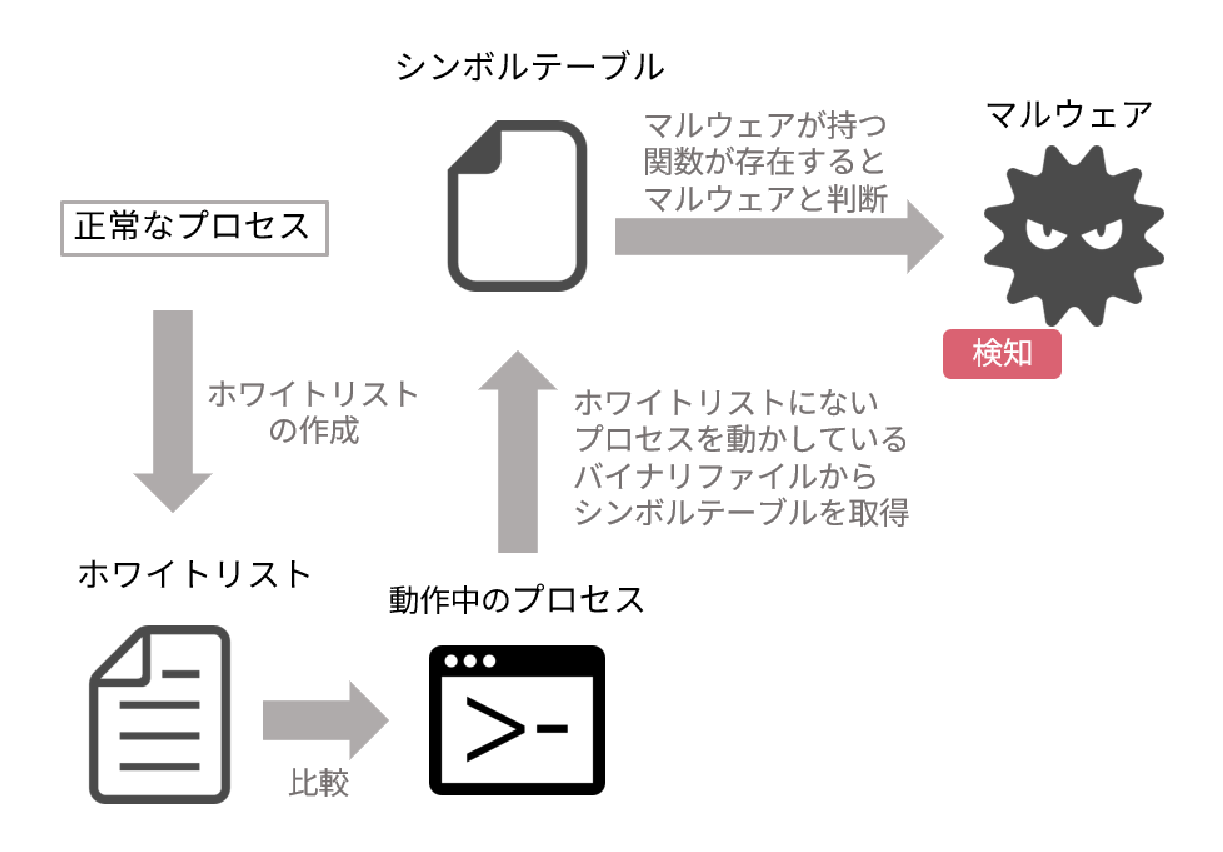
\includegraphics[width=90mm]{figures/system.eps}
 \label{fig:model}
 \begin{center}図6 検知システムの概要\end{center}
 \end{figure}
 
\section{システムコール呼び出し履歴を用いた検知手法の評価}
シンボルテーブルを用いた検知手法と同様の評価を行う.




